% chktex-file 44

\section{\large Ejercicio 6: Ejercicio Colaborativo de Equivalencia de Conceptos.}

Cada miembro del grupo deberá resolver el ejercicio correspondiente a su literal de manera individual. Luego, se les solicita realizar su aporte en el foro, compartiendo los resultados obtenidos. Además, cada integrante debe responder a la pregunta planteada al final del ejercicio.

Considere el sistema de tres ecuaciones lineales con tres incógnitas:

\[
    \begin{array}{l}
        2x_1-x_2+2x_3=6 \\
        3x_1+2x_2-x_3=4 \\
        8x_1+6x_2-6x_3=2
    \end{array}
\]

Compruebe la existencia de un vector $\vec{x}$ de $\mathbb{R}^3$, tal que $\vec{Ax}$ = $\vec{b}$ utilizando el método de eliminación de Gauss y sustitución hacia atrás.

\[
    \begin{aligned}
        \left(
            \begin{array}{ccc|c}
                2 & -1 & 2 & 6 \\
                3 & 2 & -1 & 4 \\
                8 & 6 & -6 & 2 \\
            \end{array}
        \right) & \frac{f1}{2} \\ \\
        \left(
            \begin{array}{ccc|c}
                1 & -\frac{1}{2} & 1 & 3 \\
                3 & 2 & -1 & 4 \\
                8 & 6 & -6 & 2 \\
            \end{array}
        \right) & -3f1+f2 \\ \\
        \begin{array}{ccc|c}
            -3 & \frac{3}{2} & -3 & -9 \\
            3 & 2 & -1 & 4 \\
            \hline
            0 & \frac{7}{2} & -4 & -5 \\
        \end{array} & =
        \left(
            \begin{array}{ccc|c}
                1 & -\frac{1}{2} & 1 & 3 \\
                0 & \frac{7}{2} & -4 & -5 \\
                8 & 6 & -6 & 2 \\
            \end{array}
        \right) & -8f1+f3 \\
    \end{aligned}
\]

\[
    \begin{aligned}
        \begin{array}{ccc|c}
            -8 & 4 & -8 & -24 \\
            8 & 6 & -6 & 2 \\
            \hline
            0 & 10 & -14 & -22 \\
        \end{array} & =
        \left(
            \begin{array}{ccc|c}
                1 & -\frac{1}{2} & 1 & 3 \\
                0 & \frac{7}{2} & -4 & -5 \\
                0 & 10 & -14 & -22 \\
            \end{array}
        \right) & \frac{f2}{\frac{7}{2}} \\ \\
        \left(
            \begin{array}{ccc|c}
                1 & -\frac{1}{2} & 1 & 3 \\
                0 & 1 & -\frac{8}{7} & -\frac{10}{7} \\
                0 & 10 & -14 & -22 \\
            \end{array}
        \right) & = -10f2+f3 \\ \\
        \begin{array}{ccc|c}
            0 & -10 & \frac{80}{7} & \frac{100}{7} \\
            0 & 10 & -14 & -22 \\
            \hline
            0 & 0 & -\frac{18}{7} & -\frac{54}{7} \\
        \end{array} & =
        \left(
            \begin{array}{ccc|c}
                1 & -\frac{1}{2} & 1 & 3 \\
                0 & 1 & -\frac{8}{7} & -\frac{10}{7} \\
                0 & 0 & -\frac{18}{7} & -\frac{54}{7} \\
            \end{array}
        \right)
    \end{aligned}
\]

\[x_1-\frac{1}{2}x_2+x_3=3\]
\[x_2-\frac{8}{7}x_3=-\frac{10}{7}\]
\[-\frac{18}{7}x_3=-\frac{54}{7}\]

\[x_3=-\frac{54}{7}\div-\frac{18}{7}=\frac{54}{18}=3\]
\[x_2-\frac{8}{7}(3)=-\frac{10}{7}\]
\[x_2-\frac{24}{7}=-\frac{10}{7}\]
\[x_2=-\frac{10}{7}+\frac{24}{7}=\frac{14}{7}=2\]

\[x_1-\frac{1}{2}(2)+3=3\]
\[x_1-1+3=3\]
\[x_1+2=3\]
\[x_1=3-2=1\]

\begin{center}
    \textbf{Solución:} $(1,2,3)$ 
\end{center}

\newpage
\textbf{Comprobación en GeoGebra}
\begin{figure}[ht!]
    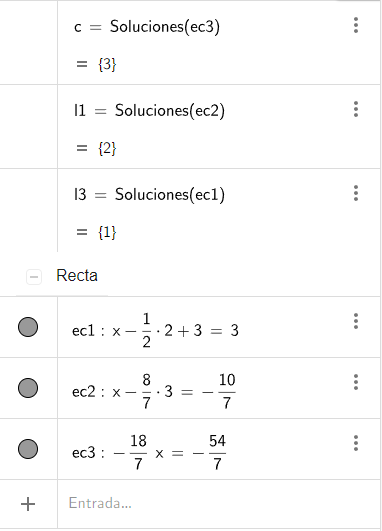
\includegraphics[width=\textwidth, height=480pt]{geogebra7.png}
\end{figure}
